%%%%%%%%%%%%%%%%%%%%%%%% ExtendedAbstract.tex %%%%%%%%%%%%%%%%%%%%%%%%
%                                                                    %
%  Extended abstract (up to 10 pages) of the MSc thesis, following   %
%  the IST template by Andre C. Marta (2011, CC BY 4.0).             %
%  Figures and references are taken from the thesis (../tese).       %
%                                                                    %
%%%%%%%%%%%%%%%%%%%%%%%%%%%%%%%%%%%%%%%%%%%%%%%%%%%%%%%%%%%%%%%%%%%%%%
\documentclass[10pt,a4paper,twocolumn]{article}

\usepackage{graphicx}
\graphicspath{{../tese/}{figures/}}
\usepackage{siunitx}

% Latin Modern for the text and the mathematics alike
\usepackage{lmodern}
\usepackage{microtype}

\usepackage[utf8]{inputenc}
\usepackage[T1]{fontenc}

% Captions in the size of the text, centred, with a plain label ("Figure 1: ..."); tables are captioned above
\usepackage[font=small, skip=4pt, labelsep=colon, justification=centering]{caption}
\usepackage[font=small]{subcaption}

\usepackage{amsmath}
\usepackage{amsfonts}
\usepackage{amssymb}
\usepackage{float}
\usepackage{placeins}
\usepackage{booktabs}
\usepackage{csquotes}

% Headings with trailing dots: sections in bold, subsections in the plain text face, both in the size of the text and
% set apart by space
\usepackage{sectsty}
\sectionfont{\normalsize\bfseries}
\subsectionfont{\normalsize\mdseries}
\usepackage{titlesec}
\titlespacing*{\section}{0pt}{12pt}{6pt}
\titlespacing*{\subsection}{0pt}{9pt}{5pt}

% Paragraphs separated by space rather than indented
\usepackage[skip=4pt plus 1pt, indent=0pt]{parskip}
\usepackage{secdot}
\sectiondot{subsection}
\sectionpunct{section}{. }
\sectionpunct{subsection}{. }

% A4 page with top margin of 25 mm, bottom of 30 mm, left and right of 25 mm (printable area 242 x 160 mm)
\setlength{\topmargin}{-10.4mm}
\setlength{\headheight}{0.0mm}
\setlength{\headsep}{10.0mm}
\setlength{\textwidth}{160mm}
\setlength{\textheight}{242mm}
\setlength{\oddsidemargin}{0mm}
\setlength{\evensidemargin}{0mm}
\setlength{\marginparwidth}{0mm}
\setlength{\marginparsep}{0mm}
\setlength{\columnsep}{6mm}

\newcommand{\eqnref}[1]{Eq.~(\ref{#1})}

% Compact bibliography: entries without extra space between them
\usepackage{etoolbox}
\apptocmd{\thebibliography}{\setlength{\itemsep}{1pt}\setlength{\parsep}{0pt}}{}{}

% Up to two full-width floats at the top of a page, so that they stay close to their text
\setcounter{dbltopnumber}{2}
\renewcommand{\dbltopfraction}{0.8}
\renewcommand{\dblfloatpagefraction}{0.8}
\renewcommand{\topfraction}{0.85}
\renewcommand{\bottomfraction}{0.7}
\renewcommand{\textfraction}{0.1}
% the figures of the results are all placed before the conclusions (\FloatBarrier), and the columns are not stretched
% to the bottom of the page when one ends before it
\raggedbottom

% Title, author and address
\title{Cooperative Control of a Tethered Drone and Surface Vessel for Sustained Presence at Sea}
\date{January 2026}
\author{Tomás Grossinho Esteves \\ tomasesteves03@gmail.com \\ \\ Instituto Superior Técnico, Lisboa, Portugal}

\begin{document}

\twocolumn[
\begin{@twocolumnfalse}
\maketitle
% Abstract and keywords (the same as in the thesis)
\begin{abstract}
An unmanned surface vessel (USV) and an unmanned aerial vehicle (UAV) connected by a tether combine the endurance of the USV with the view from above of the UAV, which draws power and a reliable communication link through the tether. The tether, however, couples the two vehicles, which must remain within its reach while each respects its own limits, under waves and wind. This work develops the cooperative control of such a system. Models of both vehicles are derived and validated against a simulator, together with a closed-form model of the force of a slack tether. Each vehicle is driven by its own non-linear model predictive controller, and the two controllers exchange their predicted trajectories, so that each anticipates the motion of the other within the reach of the tether. In a simulation at sea, each controller tracks the trajectory given to its vehicle with an error of a few centimetres, also under wind, and, when the reference cannot be followed, both keep their vehicles within their limits and the tether within its reach. The UAV lands on the moving deck a few centimetres from the centre of the pad in waves of up to $1.2\,\text{m}$ and winds of up to $8\,\text{m/s}$, and the two vehicles operate as a single system to perform missions.
\end{abstract}

\begin{IEEEkeywords}
Cooperative control, non-linear model predictive control, tether, unmanned aerial vehicle, unmanned surface vessel
\end{IEEEkeywords}

\end{@twocolumnfalse}
]

\section{Introduction}
\label{sec:intro}

% Why a USV and a UAV joined by a tether?
Saving lives at sea, protecting marine ecosystems and securing maritime infrastructure all rely on a continuous and local awareness of what happens at sea~\cite{europeanmaritimesafetyagencyEMSAOutlook2025_v302025}. Surface vessels provide a long-lasting presence, but they only see as far as the horizon, while unmanned aerial vehicles (UAVs) sense from above but have a short endurance and an unreliable long-range link~\cite{zeng2016uav,kishk2020tethered}. An unmanned surface vehicle (USV) and a UAV working as a team can keep an awareness that neither achieves alone, and a tether between them supplies the UAV with power and a reliable communication link from the vessel, which removes the two main limits of maritime UAVs~\cite{kishk2020tethered}. Such systems already exist in industry~\cite{exail_elistair_tethered,acua_ocean_teledyne_mod}, but their operation remains largely manual.

% What makes this system hard to control?
The tether, however, turns the two vehicles into a single system. The distance between them must stay within its reach, so the motion of one restricts that of the other, and the two move on very different time scales, the USV slowly, dominated by its inertia and the drag of the water, and the UAV quickly. Wind and waves disturb both, and the UAV must take off from and land on a deck that moves with the waves. In the literature, the two vehicles are often controlled separately, the tether is simplified, or the vessel is assumed to be fixed.

% What does this work do, and what does it contribute?
This work addresses the control of a USV, the WAM-V, and a UAV, the x500 multirotor, connected by a tether, so that they carry out maritime missions autonomously as a single system, each within its own limits and both within the reach of the tether, also under waves and wind. Its main contributions are:
\begin{itemize}
    \setlength{\itemsep}{0pt}
    \item control-oriented models of both vehicles and a closed-form model of the force of a slack tether, validated against a simulator;
    \item two cooperating non-linear model predictive controllers (NMPCs), one for each vehicle, which exchange their predicted trajectories to keep the tether within its reach, and plan the motion of both vehicles from simple or unreachable references;
    \item a simulation of the tethered system at sea, with waves, the PX4 autopilot and a tether whose length is set by a winch;
    \item manoeuvres and missions for both vehicles, including the takeoff from and the landing on the moving deck, and the inspection of a structure that lies beyond the reach of the tether from any fixed point of the USV;
    \item an evaluation of the system in tracking and planning, in three missions, and under waves and wind.
\end{itemize}
Section~\ref{sec:backg} reviews related work, Section~\ref{sec:model} presents the models and the controllers, Section~\ref{sec:imple} the simulation, the validation of the models and the missions, Section~\ref{sec:resul} the results, and Section~\ref{sec:concl} concludes.

\section{Related Work}
\label{sec:backg}

\textbf{Tether models.} In tethered aerial systems, the tether is most often modelled as massless, inextensible and taut, so that it acts along the straight line between its ends, as in the buoy--UAV system of~\cite{kouraniMarineLocomotionTethered2021} and the cooperative manipulation of~\cite{novakCollaborativeObjectManipulation2024}. Alternatively, its effect is not modelled and is lumped into a disturbance estimated online and rejected by the controller~\cite{yuReducedComplexityActiveDisturbance2023}. Neither describes a slack tether, whose weight bends it into a catenary~\cite{irvine1981cable} and turns its force away from the straight line.

\textbf{Control and cooperation.} Predictive control is the common choice for the cooperation of a UAV and a USV, since it can state the coupling between them as constraints over a horizon. In~\cite{liNMPCbasedUAVUSVCooperative2023}, an NMPC drives a UAV to follow and land on a moving USV, but only the UAV is controlled and the interaction is unidirectional. In~\cite{novakCollaborativeObjectManipulation2024}, a single, centralised MPC computes the inputs of both vehicles, which imposes one horizon and one sampling time on both. In~\cite{zhangCooperativeControlFramework2025}, the USV follows a predefined path with a line-of-sight guidance law, and the UAV keeps a relative configuration with its own NMPC, in a leader--follower structure without joint optimisation.

\textbf{Planning.} Existing works either assign a predefined path to one vehicle while the other follows or supports it~\cite{zhangCooperativeControlFramework2025}, or plan both motions jointly in a centralised predictive problem~\cite{novakCollaborativeObjectManipulation2024}.

This work combines elements of these approaches. It models the force of a slack tether in closed form and compensates what the model leaves out with a disturbance observer, drives each vehicle by its own NMPC, with its own horizon and sampling time, and couples the two controllers through the exchange of their predicted trajectories, so that each anticipates the motion of the other and both plan their motion online within the limits of the tether.

\section{Modelling and Control}
\label{sec:model}

\subsection{USV Model}

The WAM-V is described in the horizontal plane by its position $(x,y)$ and heading $\psi$ in the inertial frame, and by its surge, sway and yaw velocities $(u,v,r)$ in its body frame. The kinematics are $\dot x = u\cos\psi - v\sin\psi$, $\dot y = u\sin\psi + v\cos\psi$ and $\dot\psi = r$, and the dynamics follow from Newton's and Euler's laws in the rotating body frame, with the linear-plus-quadratic hydrodynamic damping of~\cite{fossenHandbookMarineCraft2011},
\begin{equation}
\begin{aligned}
    \dot u &= \tfrac{1}{m}\big[X - (X_u + X_{uu}^{\pm}|u|)u\big] + vr, \\
    \dot v &= \tfrac{1}{m}\big[Y - (Y_v + Y_{vv}|v|)v\big] - ur, \\
    \dot r &= \tfrac{1}{I_z}\big[N - (N_r + N_{rr}|r|)r\big],
\end{aligned}
\label{eq:usv_dyn}
\end{equation}
where the quadratic surge damping $X_{uu}^{\pm}$ differs between forward and backward motion. The forces and moment $(X,Y,N)$ are produced by two azimuth thrusters, with thrusts $T_L, T_R$ and angles $\alpha_L, \alpha_R$, mounted at $(-x_{arm}, \pm y_{arm})$,
\begin{equation}
\begin{aligned}
    X &= T_L\cos\alpha_L + T_R\cos\alpha_R, \\
    Y &= T_L\sin\alpha_L + T_R\sin\alpha_R, \\
    N &= -x_{arm}(T_L\sin\alpha_L + T_R\sin\alpha_R) \\
      &\quad - y_{arm}(T_L\cos\alpha_L - T_R\cos\alpha_R).
\end{aligned}
\label{eq:usv_alloc}
\end{equation}

\subsection{UAV Model}

The x500 is described by its position $\mathbf{p} = [x,y,z]^\top$ and attitude $(\phi,\theta,\psi)$. Its acceleration results from the thrust $T$ along its body vertical axis, gravity, a linear rotor drag $d_r$ on the horizontal velocity, and the force of the tether,
\begin{equation}
    \ddot{\mathbf{p}} = \frac{T}{m}\mathbf{R}(\phi,\theta,\psi)\begin{bmatrix}0\\0\\1\end{bmatrix} - \begin{bmatrix}0\\0\\g\end{bmatrix} - \frac{d_r}{m}\begin{bmatrix}\dot x\\ \dot y\\ 0\end{bmatrix} + \frac{1}{m}\mathbf{F}_{\mathrm{tether}}.
    \label{eq:uav_dyn}
\end{equation}
The UAV is driven through its autopilot, PX4~\cite{meier2015px4}, at the attitude level. The direction of the thrust $\mathbf{z}^{\mathcal{B}}$ follows the commanded one with a time constant $\tau$ after a transport delay $\tau_d$, and the yaw follows its command with $\tau_\psi$ and $\tau_{d,\psi}$,
\begin{equation}
\begin{aligned}
    \dot{\mathbf{z}}^{\mathcal{B}} &= \tfrac{1}{\tau}\big(\mathbf{R}(\phi_{\mathrm{cmd}},\theta_{\mathrm{cmd}},\psi_{\mathrm{cmd}})|_{t-\tau_d}[0,0,1]^\top - \mathbf{z}^{\mathcal{B}}\big), \\
    \dot\psi &= \tfrac{1}{\tau_\psi}\big(\psi_{\mathrm{cmd}}(t-\tau_{d,\psi}) - \psi\big).
\end{aligned}
\label{eq:uav_att}
\end{equation}
The time constants follow from the proportional gains of the attitude controller of PX4, and the delays were identified from flights with the NMPC, $\tau_d = 0.04\,\text{s}$ and $\tau_{d,\psi} = 0.06\,\text{s}$.

\subsection{Tether Force Model}

The tether is attached to a winch on the USV, at $\mathbf{p}_v$, which keeps its length $L$ slightly longer than the distance $d = \|\mathbf{r}\|$ between its ends, $\mathbf{r} = \mathbf{p}_v - \mathbf{p}$, with a constant slack ratio $\varepsilon_0 = (L-d)/L$. A tether of linear mass $\mu$ then hangs as a catenary, and the tension at the UAV is close to the weight of the tether, $T_{\mathrm{tether}} \approx \mu g L$, so that
\begin{equation}
    T_{\mathrm{tether}} = c_d\,d, \qquad c_d = \frac{\mu g}{1-\varepsilon_0}.
    \label{eq:tether_tension}
\end{equation}
The weight of the tether also turns its force away from the chord $\hat{\mathbf{d}}_0 = \mathbf{r}/d$, towards the vertical, by an angle $\gamma$. Since only the weight normal to the chord bends the tether, this deflection is largest for a horizontal chord, where it equals the angle $\gamma_0$ of the catenary at its ends, and vanishes for a vertical one, so it is taken as $\gamma = \gamma_0\cos\alpha$, where $\alpha$ is the depression angle of the chord below the horizontal direction $\hat{\mathbf{e}}_h$ in the plane of the catenary. The force on the UAV is then
\begin{equation}
    \mathbf{F}_{\mathrm{tether}} = c_d\,d\,\big[\cos(\alpha+\gamma)\,\hat{\mathbf{e}}_h - \sin(\alpha+\gamma)\,\mathbf{z}^{\mathcal{I}}\big],
    \label{eq:tether_force}
\end{equation}
a closed-form expression of the positions of the two vehicles, smooth for every orientation of the chord, which replaces the numerical solution of the catenary at every step of the controller.

\subsection{Cooperative NMPC}

Each vehicle is driven by its own NMPC, which solves, at every sampling instant $k$, an optimal control problem over a horizon of $N$ steps,
\begin{equation}
\begin{aligned}
    \min_{\hat{\mathbf{x}},\hat{\mathbf{u}},\hat{\boldsymbol\sigma}} \;& \sum_{i=0}^{N-1}\ell(\hat{\mathbf{x}}_{i},\hat{\mathbf{u}}_{i}) + \ell_f(\hat{\mathbf{x}}_{N}) + \sum_{i} \rho(\hat{\boldsymbol\sigma}_{i}) \\
    \text{s.t.}\;& \hat{\mathbf{x}}_{0} = \mathbf{x}_k, \quad \hat{\mathbf{x}}_{i+1} = \boldsymbol\Phi(\hat{\mathbf{x}}_{i},\hat{\mathbf{u}}_{i}), \\
    & \hat{\mathbf{u}}_{i}\in\mathcal{U}, \quad h_j(\hat{\mathbf{x}}_{i}) \le \hat\sigma_{j,i}, \quad \hat\sigma_{j,i}\ge 0,
\end{aligned}
\label{eq:ocp}
\end{equation}
where $\boldsymbol\Phi$ integrates the model over one sampling interval with a fourth-order Runge--Kutta method. The state constraints are softened by slacks $\sigma_j$, penalised by $\rho(\sigma) = \mu_1\sigma + \mu_2\sigma^2$, so that the problem always has a solution, and large weights keep the violations close to zero whenever the constraints can be met. Both problems are written in CasADi~\cite{anderssonCasADiSoftwareFramework2019} and solved by acados~\cite{verschueren2022acados}.

A single controller for both vehicles would impose one horizon and one sampling time on vehicles that move on very different time scales, and enlarge the problem to be solved in real time. Each vehicle therefore has its own NMPC, and the two exchange the trajectories they predict, Figure~\ref{fig:overview}. Each controller then constrains the distance between the vehicles along the predicted trajectory of the other, so that it anticipates where the other vehicle is going, rather than where it is.

\begin{figure*}[t]
    \centering
    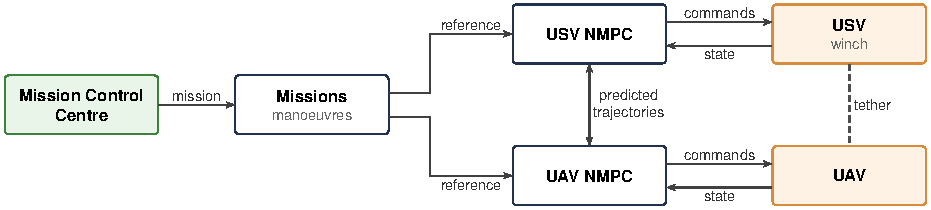
\includegraphics[width=0.62\textwidth]{Introduction/figures/system_overview.pdf}
    \caption{Overview of the system: the missions chain the manoeuvres of both vehicles, which give the references of their NMPCs, and the two controllers exchange their predicted trajectories.}
    \label{fig:overview}
\end{figure*}

\textbf{USV NMPC.} To limit both the thrusts and their rates, the thrusts and angles are included in the state, $\mathbf{x}_v = [x,y,\psi,u,v,r,T_L,T_R,\alpha_L,\alpha_R]^\top$, and the inputs are their rates, bounded by the limits of the thrusters. The stage cost penalises the errors of position, heading and velocity, $\|\mathbf{p}-\mathbf{p}_{ref}\|^2_{Q_p} + q_\psi(1-\cos(\psi-\psi_{ref})) + \|\boldsymbol\nu-\boldsymbol\nu_{ref}\|^2_{Q_\nu}$, together with the thrusts and their rates. A soft lower bound on the surge speed keeps the vessel sailing bow first, and the separation from the predicted trajectory of the UAV, $\hat{\mathbf{p}}_a$, is limited by the reach of the tether,
\begin{equation}
    (x-\hat x_a)^2 + (y-\hat y_a)^2 + (\hat z_a - z_t)^2 - d_{max}^2 \le \sigma,
    \label{eq:usv_tether}
\end{equation}
where $z_t$ is the height of the winch. The USV NMPC runs at $10\,\text{Hz}$ with a horizon of $2\,\text{s}$.

\textbf{UAV NMPC.} The commanded attitude and the thrust are included in the state, $\mathbf{x}_a = [\mathbf{p},\dot{\mathbf{p}},\phi,\theta,\psi,\phi_{\mathrm{cmd}},\theta_{\mathrm{cmd}},\psi_{\mathrm{cmd}},T]^\top$, the inputs are their rates, and the model combines \eqref{eq:uav_dyn}--\eqref{eq:tether_force}, with the tether attached to the predicted trajectory of the USV. The stage cost penalises the errors of position and velocity, the tilt, the deviation of the thrust from hover and the inputs, and keeps the UAV looking at the winch, a term that fades within about $2\,\text{m}$ of it. The soft constraints $h_1$--$h_7$ bound the height, the horizontal and vertical speeds and the tilt, which is applied to both the attitude and its command, $\max(|\phi|,|\phi_{\mathrm{cmd}}|) \le \phi_{max}$, so that the command sent to the autopilot also respects it. The tether gives the last two: the separation is limited, $d^2 \le d_{max}^2$, and so is the rate at which it grows, $\mathbf{r}^\top\dot{\mathbf{r}}/d \le \dot d_{max}$, which may not exceed the pay-out of the winch. The UAV NMPC runs at $50\,\text{Hz}$ with a horizon of $1\,\text{s}$.

\textbf{Disturbance observer.} A force that the model does not describe, such as wind, makes the prediction drift and leaves a steady offset. Following the disturbance-model approach to offset-free predictive control~\cite{pannocchia2003offsetfree,maeder2009offsetfree}, an external force $\hat{\mathbf{F}}_{\mathrm{ext}}$, held constant over the horizon, is added to \eqref{eq:uav_dyn} and estimated from the one-step prediction error of the velocity,
\begin{equation}
    \hat{\mathbf{F}}_{\mathrm{ext},k} = \mathrm{sat}_{\bar F}\Big(\hat{\mathbf{F}}_{\mathrm{ext},k-1} + \beta\frac{m}{T_s}\big(\mathbf{v}_k - \hat{\mathbf{v}}_{k|k-1}\big)\Big),
    \label{eq:observer}
\end{equation}
with a gain $\beta = 0.03$, which gives a time constant of about $T_s/\beta \approx 0.7\,\text{s}$, and a bound $\bar F = 8\,\text{N}$.

\section{Implementation}
\label{sec:imple}

\subsection{Simulation Environment}

The system is simulated in Gazebo~\cite{koenig2004gazebo}, with the hydrodynamics and the waves of the Virtual RobotX environment~\cite{bingham2019vrx}, in which the WAM-V floats on a wave field that makes it heave, roll and pitch. The x500 is flown by PX4 in software-in-the-loop, so that the NMPC drives it through the same autopilot as on the real vehicle. The tether is simulated with MoorDyn~\cite{hall2015moordyn}, as a chain of $30$ lumped masses connected by elastic segments, with the weight and the drag of the tether at the nodes, so that it hangs, goes slack and pulls on both vehicles through its own dynamics rather than through the model of the controllers. A virtual winch on the deck adjusts its length to keep the slack ratio $\varepsilon_0 = 5\,\%$, at up to $2\,\text{m/s}$, and can pull the UAV towards the deck with a constant force, to hold it during the takeoff and the landing. Wind acts on the UAV as a drag force with gusts. All the components communicate through ROS~2, and the state of both vehicles is taken from the simulator.

\subsection{Model Validation}

The models of Section~\ref{sec:model} were compared with the simulator using its nominal parameters, without fitting them to the validation data, as they are used by the controllers: over predictions of the length of each horizon, started from the state of the simulator and driven by the recorded commands. Table~\ref{tab:validation} summarises the errors at the end of the horizons. The model of the WAM-V predicts its position within $1.4\,\text{cm}$ over $2\,\text{s}$, less than $2\,\%$ of its length at the worst. The model of the x500 predicts its position within $11\,\text{cm}$ over the up to $8\,\text{m}$ it travels in $1\,\text{s}$, and the delays of the attitude response reduce the error of the attitude from about $5\,\%$ to below $1.5\,\%$ of its range. The model of the tether reduces the error of the force by $72\,\%$ and $76\,\%$ relative to a taut tether and to a hanging load, to $0.25\,\text{N}$, $1.2\,\%$ of the weight of the UAV.

\begin{table}[t]
    \centering
    \caption{Errors of the models against the simulator (RMSE, and NRMSE relative to the range of each signal).}
    \label{tab:validation}
    \footnotesize
    \begin{tabular}{@{}llrr@{}}
        \toprule
        Model & Quantity & RMSE & NRMSE \\
        \midrule
        WAM-V, $2\,\text{s}$ & position & $1.4\,\text{cm}$ & $0.37\,\%$ \\
         & heading & $0.16^\circ$ & $0.33\,\%$ \\
        x500, $1\,\text{s}$ & position & $10.8\,\text{cm}$ & $1.34\,\%$ \\
         & velocity & $0.17\,\text{m/s}$ & $2.02\,\%$ \\
         & roll, pitch & $0.63^\circ$, $0.40^\circ$ & $1.32$, $0.89\,\%$ \\
        Tether force & model & $0.25\,\text{N}$ & $10.8\,\%$ \\
         & taut tether & $0.90\,\text{N}$ & $38.9\,\%$ \\
         & hanging load & $1.03\,\text{N}$ & $44.7\,\%$ \\
        \bottomrule
    \end{tabular}
\end{table}

\subsection{Manoeuvres and Missions}

The controllers follow references, but do not decide where each vehicle should go. This is the role of the manoeuvres, which give the reference of one vehicle over the horizon of its controller at every instant. The UAV can take off, fly in formation at a point relative to the USV, in its axes or in fixed axes, orbit the USV or a point in the world, chase a target, and land, and the USV can hold its position, follow a route, pursue a target, and support the UAV from the water, following the point below it pushed away from a structure, so that it gives the UAV the reach of the tether. Since the controllers keep the vehicles within their limits, the references can remain simple, often a single point. Figure~\ref{fig:catalogue} shows the manoeuvres of the UAV as flown in the missions.

\begin{figure*}[t]
    \centering
    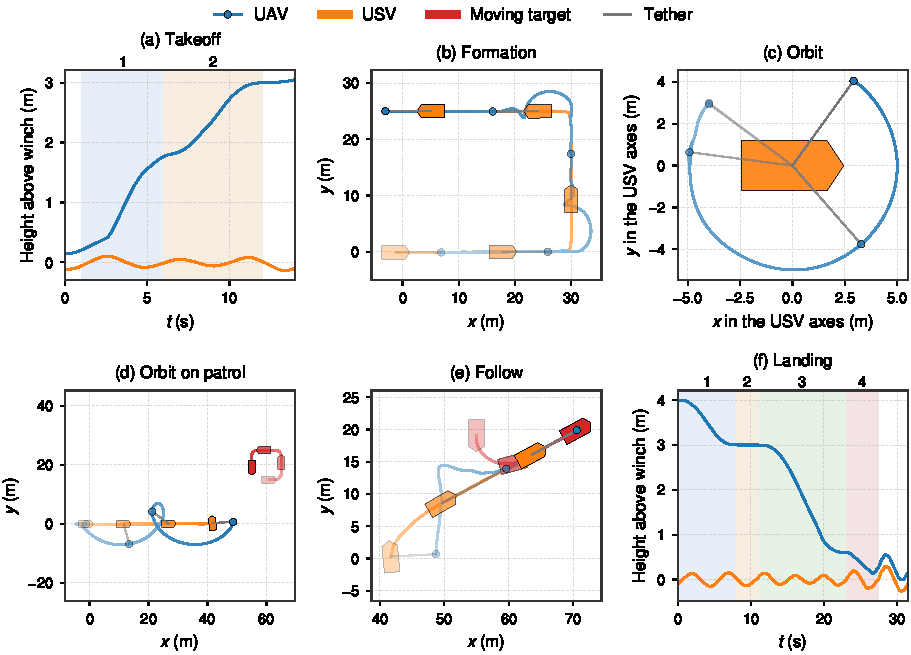
\includegraphics[width=0.85\textwidth]{Implementation/figures/04_maneuvers_and_missions/maneuver_catalogue.pdf}
    \caption{Manoeuvres of the UAV in simulation: takeoff (a) and landing (f) through the height of the UAV above the winch, with their phases, and formation (b), orbit (c, in the axes of the USV), orbit on patrol (d) and chase (e) from above, with the positions of the vehicles and the tether at several instants.}
    \label{fig:catalogue}
\end{figure*}

The takeoff and the landing are the manoeuvres in which the UAV is closest to the deck and moves with it. The takeoff starts with a vertical climb while the winch holds the UAV against the deck, so that it does not drift over its edge at low height. In the landing, the UAV first waits above the pad until it is centred and moving with it, then descends with the winch pulling it, and ends with a slow approach towards a point below the deck, so that it touches down even if the deck falls away.

A mission is a file with a sequence of manoeuvres for each vehicle, in which each manoeuvre ends with an event, such as the detection of a target, or with the end of a manoeuvre of the other vehicle. Three missions were tested: a scout, in which the UAV flies ahead of the bow while the USV follows a route, an inspection, in which the UAV circles a tower while the USV supports it, and a patrol, in which the UAV orbits the USV until it detects a target, which it then chases while the USV pursues it.

\begin{figure*}[t]
    \centering
    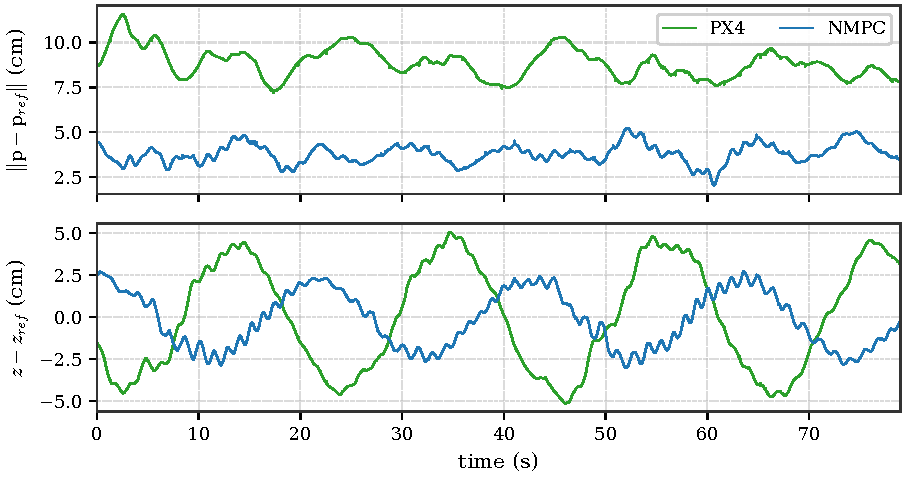
\includegraphics[width=0.8\textwidth]{Results/figures/01_tracking/nominal_error.pdf}
    \caption{Tracking error of the UAV on the tilted circle with the NMPC and with the position controller of PX4: norm of the position error and its vertical component.}
    \label{fig:nominal}
\end{figure*}

\section{Results}
\label{sec:resul}

All results were obtained in simulation, with the default sea of the simulator, which moves the winch up and down by about $0.25\,\text{m}$, without wind unless stated otherwise, and with the state of both vehicles taken from the simulator.

\begin{figure*}[t]
    \centering
    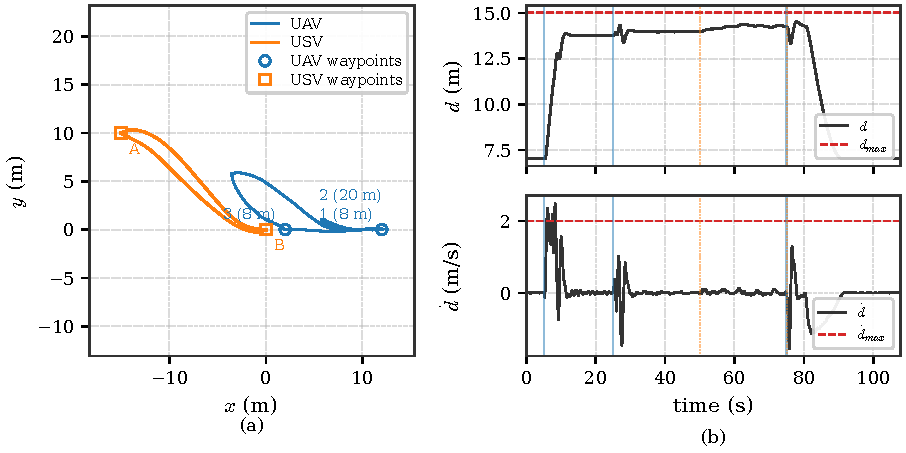
\includegraphics[width=0.8\textwidth]{Results/figures/01_tracking/steps_tether.pdf}
    \caption{Step references: (a) paths and waypoints, with the height of those of the UAV, and (b) separation $d$ and its rate $\dot d$, with their limits; vertical lines mark the steps of the UAV (solid) and of the USV (dotted).}
    \label{fig:steps}
\end{figure*}

\subsection{Tracking}

The tracking was first measured on a reference that both vehicles can follow. The USV sails a circle of $3\,\text{m}$ radius at $0.15\,\text{m/s}$, while the UAV flies a circle of $5\,\text{m}$ about the same centre at $1.5\,\text{m/s}$, tilted so that its height goes from $21$ to $29\,\text{m}$. Since the two circles are flown at different angular speeds, the separation varies between $20$ and $29\,\text{m}$, and so does the force of the tether, between $3.9$ and $6.0\,\text{N}$. For comparison, the same circle was also flown by the position controller of PX4, which receives the position, velocity and acceleration of the reference, is not aware of the tether, and compensates constant forces through the integral action of its velocity loop.


Figure~\ref{fig:nominal} and Table~\ref{tab:nominal} show that the NMPC follows the circle with less than half the error of PX4, $4.0$ against $9.0\,\text{cm}$. Neither keeps an offset in height, and the difference lies in the timing: PX4 reacts to the error once it has appeared, and follows the reference about $45\,\text{ms}$ behind it, while the NMPC anticipates its motion over the horizon. The USV follows its circle within $0.6\,\text{cm}$, and the two NMPCs take on average $4.8$ and $1.9\,\text{ms}$ of their sampling periods of $20$ and $100\,\text{ms}$.

\begin{table}[t]
    \centering
    \caption{Position error of the UAV on the tilted circle (cm), over $68\,\text{s}$.}
    \label{tab:nominal}
    \footnotesize
    \begin{tabular}{@{}lrrrrr@{}}
        \toprule
        Controller & RMSE & Max. & $x$ & $y$ & $z$ \\
        \midrule
        NMPC & $4.0$ & $5.3$ & $2.6$ & $2.5$ & $1.7$ \\
        PX4 & $9.0$ & $11.6$ & $5.9$ & $5.9$ & $3.2$ \\
        \bottomrule
    \end{tabular}
\end{table}

\begin{figure*}[t]
    \centering
    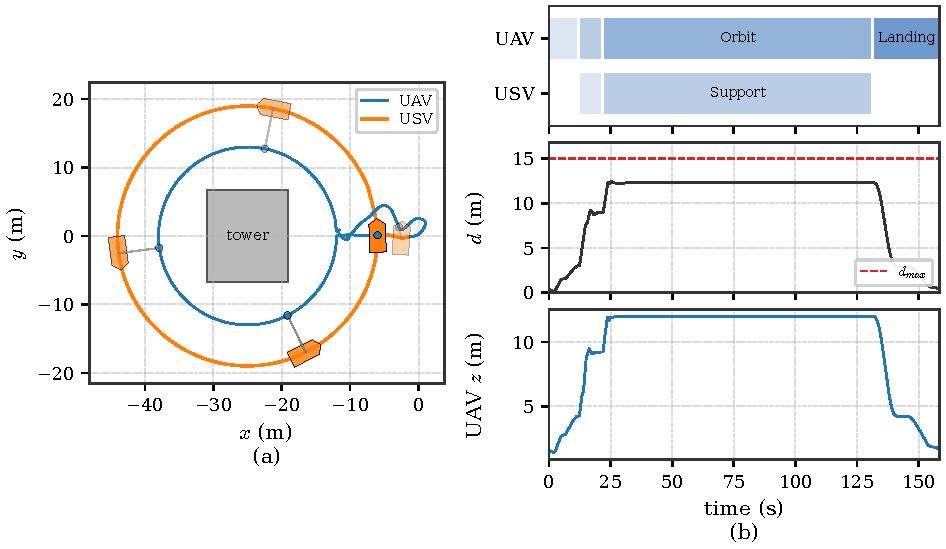
\includegraphics[width=0.85\textwidth]{Results/figures/02_missions/inspection.pdf}
    \caption{Inspection mission: (a) paths of both vehicles around the tower, with their positions and the tether at five instants, and (b) manoeuvres of each vehicle, separation $d$ and height of the UAV.}
    \label{fig:inspection}
\end{figure*}

\subsection{Planning}

To test the planning, both vehicles were given step references, single points held fixed over the horizon, with $d_{max} = 15\,\text{m}$. The UAV is sent $10\,\text{m}$ sideways, then $12\,\text{m}$ up, to a point $22\,\text{m}$ from the winch, beyond the reach of the tether; the USV is then sent $18\,\text{m}$ away, and both finally return, Figure~\ref{fig:steps}.


When its reference lies beyond the reach of the tether, the UAV stops short of it, on the line towards it, at $14\,\text{m}$ from the winch, and when the USV then sails away, it follows the USV, with the separation between $14.0$ and $14.4\,\text{m}$. In the first step, moving sideways at the same height would separate the vehicles faster than the winch pays out the tether, and the UAV drops by $2\,\text{m}$ on the way to slow the growth of the separation, whose rate exceeds its limit of $2\,\text{m/s}$ only briefly at the start of the step. The steps bring the actuators to their limits: the thrust of the UAV saturates at its maximum and its commanded tilt at $28.6^\circ$, while the thrusters of the USV reach their maximum reverse thrust and their maximum angle as it turns in place. The rates of all the commands reach their limits without exceeding them, and the real pitch of the UAV exceeds its limit by at most $1.7^\circ$, as the attitude loop of the autopilot slightly overshoots its command. The controllers therefore do not need feasible, or even continuous, references, which keeps the manoeuvres simple.


\begin{figure*}[t]
    \centering
    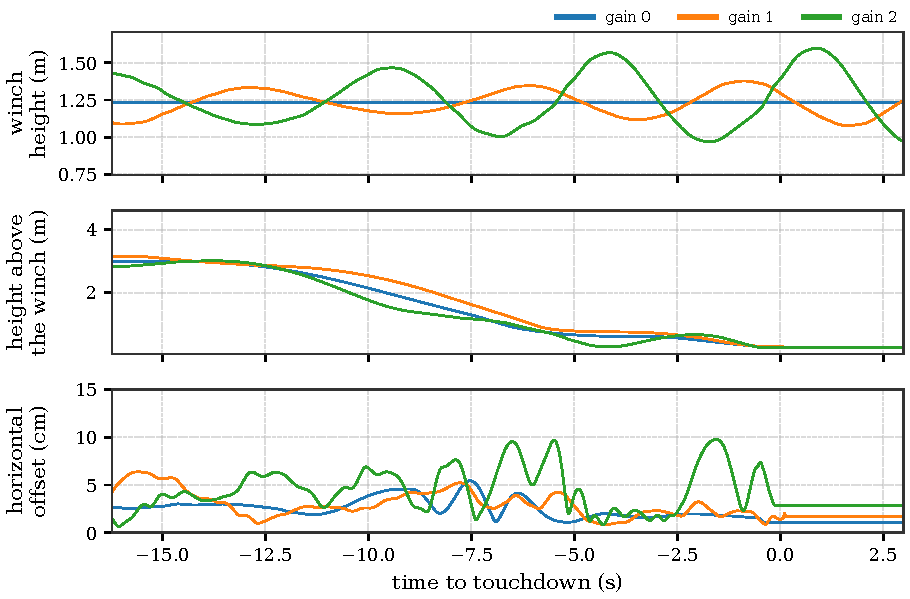
\includegraphics[width=0.7\textwidth]{Results/figures/03_disturbances/waves_landing.pdf}
    \caption{Landing with waves, from the start of the descent to the touchdown: height of the winch, height of the UAV above it, and horizontal offset from it.}
    \label{fig:waves}
\end{figure*}

\begin{figure*}[t]
    \centering
    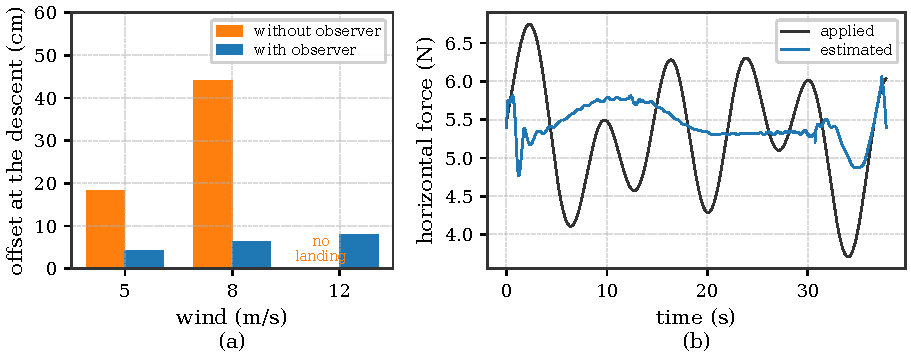
\includegraphics[width=0.8\textwidth]{Results/figures/03_disturbances/wind.pdf}
    \caption{Landing with wind: (a) offset of the UAV from the winch when the descent starts, and (b) force of a $12\,\text{m/s}$ wind and estimate of the observer.}
    \label{fig:wind}
\end{figure*}

\subsection{Missions}

The three missions were flown with $d_{max} = 15\,\text{m}$, and are summarised in Table~\ref{tab:missions}. In the scout, the UAV keeps $8\,\text{m}$ ahead of the bow of the USV as it sails a route with two turns of $90^\circ$, with a mean error of $5\,\text{cm}$, largest at the turns, where the point ahead of the bow swings around the USV. In the patrol, the UAV detects a fleeing target $19\,\text{m}$ away, beyond the reach of the tether; its reference is brought within reach along the line from the USV, which lowers it, and the UAV is above the target $5\,\text{s}$ after the detection, while the USV, at up to $2.2\,\text{m/s}$, catches up with it $21\,\text{s}$ after the detection.


The inspection, Figure~\ref{fig:inspection}, shows best how the two vehicles work as one system. The UAV circles a tower of $12$ by $13\,\text{m}$ at a radius of $13\,\text{m}$, a circle beyond the reach of the tether from any fixed point. Its reference is a circle fixed in the world, regardless of the USV, while the USV supports it from the water, $6\,\text{m}$ further from the tower. The USV keeps within $3\,\text{cm}$ of its intended radius around the whole tower, the separation stays at $12.3\,\text{m}$, and the UAV follows its circle within $1\,\text{cm}$, so that the two vehicles together cover a circle that neither could cover alone.

\begin{table}[t]
    \centering
    \caption{Missions with $d_{max} = 15\,\text{m}$: duration, largest separation, and distance of the touchdown from the centre of the pad.}
    \label{tab:missions}
    \footnotesize
    \begin{tabular}{@{}lrrr@{}}
        \toprule
        Mission & Duration & Max. $d$ & Touchdown \\
        \midrule
        Scout & $132\,\text{s}$ & $9.6\,\text{m}$ & $3\,\text{cm}$ \\
        Inspection & $159\,\text{s}$ & $12.5\,\text{m}$ & $4\,\text{cm}$ \\
        Patrol & $104\,\text{s}$ & $14.7\,\text{m}$ & $5\,\text{cm}$ \\
        \bottomrule
    \end{tabular}
\end{table}

\subsection{Waves and Wind}

The disturbances were added during the landing on the deck of the USV, sailing a route at $0.75\,\text{m/s}$. With the gain of the wave field raised to $1$ and $2$, the winch rises and falls by $0.25$ and $0.44\,\text{m}$, Figure~\ref{fig:waves}. The landing takes the same $25$ to $27\,\text{s}$ in all sea states, since the reference is taken above the mean height of the winch, and the UAV touches down $0$, $2$ and $4\,\text{cm}$ from the centre of the pad. What the waves change is the contact: the final approach aims below the deck, so the speed of the contact is set by its motion, and grows from $0.15$ to $0.26$ and $0.39\,\text{m/s}$.


The wind was applied as a drag force on the UAV, with means of $0.9$, $2.4$ and $5.3\,\text{N}$ for $5$, $8$ and $12\,\text{m/s}$ and gusts of $\pm 30\,\%$, with and without the disturbance observer, Figure~\ref{fig:wind}. Without the observer, the UAV settles away from its reference, $18$, $44$ and $83\,\text{cm}$ from the centre of the pad before the descent, the landing waits for a centring that never happens, and at $12\,\text{m/s}$ the mission failed in both runs, once at the takeoff and once when the UAV, landing $0.8\,\text{m}$ off the centre, was blown off the edge of the pad. With the observer, whose estimate follows the force of the wind about $0.7\,\text{s}$ behind it, gusts included, the offset is $4$, $6$ and $19\,\text{cm}$ and the UAV lands within $8\,\text{cm}$ of the centre. The most exposed moment is then the takeoff, when a strong crosswind can tip the UAV against the pad while the winch still holds it, before the controller has any effect; the NMPC recovers it once it is released, after a drift of $5.5\,\text{m}$.


\section{Conclusions}
\label{sec:concl}

% What was achieved?
This work set out to operate a USV and a UAV connected by a tether as a single system at sea, each vehicle within its own limits and both within the reach of the tether. Models of both vehicles, derived from their physics and validated against the simulator, predict their motion over the horizons of the controllers with errors of a few percent, and a closed-form model of a slack tether that accounts for its weight reduces the error of its force by about three quarters relative to a taut tether or a hanging load. On these models, each vehicle is driven by its own NMPC, and the two exchange the trajectories they predict, so that each keeps the separation within the reach of the tether while anticipating where the other vehicle is going.

% What do the results show?
Both controllers track the trajectories given to their vehicles within a few centimetres, the UAV more than four times closer than the position controller of PX4, and with nearly the same error under a wind of $8\,\text{m/s}$, which the disturbance observer compensates. When a reference demands more than a vehicle can deliver, each controller gives up following it only as far as the limits require, and the separation between the vehicles is held at the reach of the tether, so that any trajectory can be given to either vehicle without putting the tether at risk, and the manoeuvres can remain simple. The UAV lands on the moving deck a few centimetres from the centre of the pad in every sea tested, with a speed of contact that grows with the waves and in the higher sea reaches the default landing speed of PX4, and, with the disturbance observer, also under wind, which otherwise forces the landing to be aborted. Coupled by the tether, the two vehicles complete an inspection, a patrol and a recovery as a single system, and in the inspection the tether becomes not a constraint to be avoided, but a means to survey a tower that neither vehicle could survey alone.

% What comes next?
The system was developed and evaluated in simulation, and bringing it to real operations at sea is a long path. Its main steps are the hardware of the tethered system, with RTK receivers on both vehicles that also give their relative position, the validation of the models and the estimation of the state on the real vehicles, the handling of failures and the avoidance of obstacles, which may require longer horizons, and a gradual validation from land to the open sea, where a prediction of the motion of the deck could time the touchdown. Even then, a much larger volume of testing would be needed before real use.


{\footnotesize
\bibliographystyle{abbrv}
\bibliography{../tese/refs}}

\end{document}
